\documentclass[12pt,a5paper,landscape]{scrartcl}

\usepackage{vorschule}
\usepackage[
    typ=ohne,
    fach=Mathematik,
    lerngruppe={6},
	nummer=2,
    module={Lizenzen,Symbole},
	seitenzahlen=keine,
	farbig,
    lizenz=cc-by-nc-sa-4,
]{schule}

\usepackage[
	typ=lerntheke,
	kuerzel=Ngb,
	reihe={Dezimalzahlen},
	version={2020-02-12},
]{ngbschule}

\author{J. Neugebauer}
\title{Dezimalzahlen}
\date{\Heute}

\begin{document}

	\begin{hilfekarte}{Dezimalzahlen}{dezimalzahlen}

	\end{hilfekarte}
	
	\begin{hilfekarte}{Brüche umwandeln}{umwandeln}
		Manchmal ist es wichtig zu wissen, wie ein Bruch in einen Dezimalbruch umgewandelt werden kann. Maik bestellt bei einem Metzger $\tSI{1}{4}{\kilo\gram}$ Hackfleisch, wie viel Kilogramm sind das? 
		
		Um dies zu lösen kannst du zwei Methoden verwenden.
		\begin{enumerate}
			\item Erweitere oder kürze den Nenner auf 10, 100, 1000 usw. Beispiel:
			
			\[ \dfrac{1}{4} = \dfrac{25	}{100} = 0,25 \]
			\item Wandle einen Bruch durch schriftliche Division in einen Dezimalbruch um. Beispiel:
			
			\[ \dfrac{1}{4} = \longdivision{1}{4} \]
		\end{enumerate}
	\end{hilfekarte}
			
	\begin{hilfekarte}{Abbrechende und periodische Dezimalzahlen}{abbrechend-und-periodisch}

	\end{hilfekarte}
	
	\begin{hilfekarte}{Runden und überschlagen}{runden}
		Gerade beim Einkaufen ist es hilfreich, dass du mit gerundeten Zahlen schnell die ungefähre Summe \textbf{überschlagen} kann. Rundet dabei immer so, dass du leicht im Kopf rechnen kannst.
		
		Runden von Dezimalbrüchen:
		\begin{smallenumerate}
			\item Lege die Stelle fest, auf die gerundet werden soll (Zehntel, Hundertstel, Tausendstel).
			\item Betrachte die nächstfolgende Ziffer:
			\begin{smallitemize}
				\item Ist die Ziffer 0, 1, 2, 3 oder 4, so \textbf{rundest} du \textbf{ab}.
				\item Ist die Ziffer 5, 6, 7, 8 oder 9, so \textbf{rundest} du \textbf{auf}.
			\end{smallitemize}
		\end{smallenumerate}
		
		\begin{wrapfig}
			\begin{wrapfigure}[12]{r}{0pt}		
				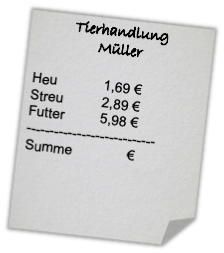
\includegraphics[width=3cm]{6.2-LT-Abb_Kassenzettel_0}
			\end{wrapfigure}
			\textbf{Beispiel:} Sonja kauft für ihr Meerschweinchen ein. An der Kasse stellt sie fest, dass sie nur \SI{11}{ Euro} bei sich hat. Um zu überschlagen, ob das Geld reicht, rundet sie die Beträge auf und rechnet $2+3+6=11$. Sie weiß nun, dass sie etwas weniger als \EUR{11} zahlen muss.
		\end{wrapfig}
	\end{hilfekarte}
	
	\begin{hilfekarte}{Dezimalzahlen ordnen}{ordnen}

	\end{hilfekarte}
	
	\begin{hilfekarte}{Addition und Subtraktion}{addition-und-subtraktion}
		\begin{wrapfigure}{r}{0pt}		
			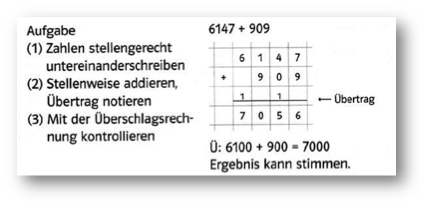
\includegraphics[height=.45\textheight]{6.2-LT-Abb_Addition}
		\end{wrapfigure}
		
		
		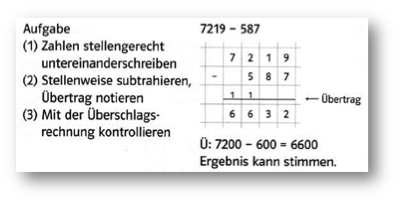
\includegraphics[height=.45\textheight]{6.2-LT-Abb_Subtraktion}
	\end{hilfekarte}
	
	\begin{hilfekarte}{Multiplikation und Division}{multiplikation-und-division}
		Du multiplizierst zwei Dezimalzahlen, indem du die Zahlen zuerst ohne Komma multiplizierst. Verschiebe dann das Komma im Ergebnis um die Anzahl der Nachkommastellen (NKS) nach links, die beide Faktoren zusammen haben (zum Beispiel um vier Stellen, wenn der erste Faktor eine NKS und der zweite drei hat).
		\[
		\underbrace{4,2}_{\text{1 NKS}}\cdot \underbrace{3,1}_{\text{1 NKS}} = \underbrace{13,02}_{\text{2 NKS}} \qquad 
		\underbrace{0,003}_{\text{3 NKS}}\cdot \underbrace{5}_{\text{0 NKS}} = \underbrace{0,015}_{\text{3 NKS}} \qquad
		\underbrace{0,06}_{\text{2 NKS}}\cdot \underbrace{0,05}_{\text{2 NKS}} = \underbrace{0,0030}_{\text{4 NKS}}
		\]
		
		Du \emph{dividierst} zwei Dezimalzahlen, indem du das Komma in beiden Zahlen um dieselbe Anzahl stellen nach rechts verschiebt, so dass die zweite Zahl (der Divisor) keine NKS mehr hat. Das Ergebnis bleibt dabei gleich. 
		Dann kannst du wie gewohnt schriftlich dividieren. Vergiss dabei nicht, das Komma zu setzen.
		\[ 4,08 : 2,4 = 40,8 : 24 \qquad \longdivision{40.8}{24} \]
	\end{hilfekarte}
	
	
	\begin{karte1}{Überschlagrechnung}\hilfeMarke{runden}
	Im Alltag muss man oft Kosten abschätzen. Wenn es schnell gehen soll, kann man eine \emph{Überschlagsrechnung} durchführen.

	\smallskip
	\textbf{Beispiel:} statt \EUR{5,10} + \EUR{12,98} + \EUR{7,90} rechne \EUR{5} + \EUR{13} + \EUR{8} = \EUR{26} also \EUR{5,10} + \EUR{12,98} + \EUR{7,90} $\approx$ \EUR{26}

	\smallskip
	Überschlage und runde auf ganze Euro.
	\begin{enumeratea}
		\item \EUR{2,98} + \EUR{17,05} + \EUR{4,95} $\approx$ \linie[1cm]
		\item \EUR{14,90} - \EUR{6,10} - \EUR{2,95} $\approx$ \linie[1cm]
		\item \EUR{23,89} - \EUR{8,90} + \EUR{3,99} $\approx$ \linie[1cm]
		\item 3$\cdot$ \EUR{4,99} + 7$\cdot$ \EUR{3,19} $\approx$ \linie[1cm]
	\end{enumeratea}
	\end{karte1}
	
	\begin{loesungskarte}
	\begin{enumeratea}
		\item \EUR{2,98} + \EUR{17,05} + \EUR{4,95} $\approx$ \EUR{3} + \EUR{17} + \EUR{5} = \EUR{25}
		\item \EUR{14,90} - \EUR{6,10} - \EUR{2,95} $\approx$ \EUR{15} - \EUR{6} - \EUR{3} = \EUR{6}
		\item \EUR{23,89} - \EUR{8,90} + \EUR{3,99} $\approx$ \EUR{24} - \EUR{9} + \EUR{4} = \EUR{19}
	\end{enumeratea}
	\end{loesungskarte}
	
	\begin{karte1}{Addieren und Subtrahieren}\hilfeMarke{addition-und-subtraktion}
		Berechen die Lösungen der Aufgaben.
		
		\begin{tasks}(3)
			\task $1,59 + 1,7$
			\task $4,77 + 2,24$
			\task $2,612 + 1,182$
			
			\task $5,51 - 3,00$
			\task $9,19 - 6,86$
			\task $6,427 - 5,907$
			
			\task $8,84 + 28,2 + 0,611$
			\task $6,17 - 0,879 - 1,72$
			\task $7,2918 + 4,1452 + 5,7415$
			
			\task $2,5055 + 6,0773 - 2,7586$
			\task $9,3927 - 4,2577 + 3,5623$
		\end{tasks}
	\end{karte1}
	
	\begin{loesungskarte}
		\begin{tasks}(3)
			\task $3,29$
			\task $7,01$
			\task $3,794$
			
			\task $2,51$
			\task $2,33$
			\task $0,52$
			
			\task $37,651$
			\task $3,571$
			\task $17,1785$
			
			\task $5,8242$
			\task $8,6973$
		\end{tasks}
	\end{loesungskarte}
	
	\begin{karte1}{Multiplizieren und Dividieren}\hilfeMarke{multiplikation-und-division}
			Berechen die Lösungen der Aufgaben.
			
			\begin{tasks}(3)
				\task $1,59 + 1,7$
				\task $4,77 + 2,24$
				\task $2,612 + 1,182$
				
				\task $5,51 - 3,00$
				\task $9,19 - 6,86$
				\task $6,427 - 5,907$
				
				\task $8,84 + 28,2 + 0,611$
				\task $6,17 - 0,879 - 1,72$
				\task $7,2918 + 4,1452 + 5,7415$
				
				\task $2,5055 + 6,0773 - 2,7586$
				\task $9,3927 - 4,2577 + 3,5623$
			\end{tasks}
	\end{karte1}
	
	\begin{loesungskarte}
	\end{loesungskarte}
	
	\begin{karte2}[\symUhr]{Rechnen auf Zeit}
		\begin{wrapfig}
			\begin{wrapfigure}[4]{r}{0pt}
				
\includegraphics[width=2cm]{6.2-LT-Abb_Stoppuhr}
			\end{wrapfigure}
			Berechne die Lösung der Aufgaben \emph{möglichst schnell}. Stopp deine Zeit mit einer Uhr oder deinem Handy. Schaffst du all Aufgaben in 10 Minuten?
		\end{wrapfig}
		
		\begin{tasks}(2)
			\task $5,62\cdot  3,42$
			\task $(12,23 - 10,22)\cdot 4,1$
			\task $17,433 + 5,2\cdot 3,41$
			\task $2,35 : 0,5 + 1,3$
			\task $\dfrac{3}{5} + 3,46 - \dfrac{1}{10}$
			\task $4,55 + \dfrac{1}{20}- 0,4$
		\end{tasks}
		
		\infotext{\enquote{Chronometer} von \url{http://schulbilder.org}}
	\end{karte2}
	
	\begin{loesungskarte}
		\begin{tasks}(2)
			\task $19,2204$
			\task $8,241$
			\task $35,165$
			\task $6$
			\task $3,96$
			\task $4,2$
		\end{tasks}
	\end{loesungskarte}
	
	\begin{karte1}{Kontoauszüge}
		Berechne das grau markierte Feld im Kontoauszug.
		
		\begin{multicols}{2}\footnotesize\centering
		
		\begin{tabular}{|l|l|r|} \hline
		\multicolumn{2}{|l}{\small\textbf{Sparkasse Ranstadt}} & Kontonr.: 1487523 \\ \hline
		\multicolumn{2}{|r|}{\texttt{Alter Kontostand:}} & +\color{green!50!black}\EUR{52,71} \\ \hline
		\textbf{Datum} & \textbf{Art} & \textbf{Betrag} \\ \hline
		2.2.19 & Gehalt & +\color{green!50!black}\EUR{2012,54} \\ \hline
		3.2.19 & Einzahlung & +\color{green!50!black}\EUR{124,95} \\ \hline
		5.2.19 & Zinsgutschrift & +\color{green!50!black}\EUR{741,69} \\ \hline
		\multicolumn{2}{|r|}{\texttt{Neuer Kontostand:}} & \cellcolor{lightgray} \\ \hline
		\end{tabular}
		
		\medskip
		\begin{tabular}{|l|l|r|} \hline
		\multicolumn{2}{|l}{\small\textbf{Sparkasse Hungen}} & Kontonr.: 657485420 \\ \hline
		\multicolumn{2}{|r|}{\texttt{Alter Kontostand:}} & +\color{green!50!black}\EUR{2874,11} \\ \hline
		\textbf{Datum} & \textbf{Art} & \textbf{Betrag} \\ \hline
		12.3.19 & Miete & -\color{red}\EUR{1255,68} \\ \hline
		14.3.19 & Bausparen & -\color{red}\EUR{457,21} \\ \hline
		16.3.19 & Krankenversicherung & -\color{red}\EUR{298,61} \\ \hline
		20.3.19 & Überweisung & -\color{red}\EUR{317,04} \\ \hline
		\multicolumn{2}{|r|}{\texttt{Neuer Kontostand:}} & \cellcolor{lightgray} \\ \hline
		\end{tabular}
		
		\columnbreak
		
		\begin{tabular}{|l|l|r|} \hline
		\multicolumn{2}{|l}{\small\textbf{Sparkasse Friedberg}} & Kontonr.: 25479632 \\ \hline
		\multicolumn{2}{|r|}{\texttt{Alter Kontostand:}} & +\color{green!50!black}\EUR{3457,54} \\ \hline
		\textbf{Datum} & \textbf{Art} & \textbf{Betrag} \\ \hline
		2.2.19 & Miete & -\color{red}\EUR{874,53} \\ \hline
		4.2.19 & Bausparen & -\color{red}\EUR{165,23} \\ \hline
		4.2.19 & Krankenversicherung & -\color{red}\EUR{456,87} \\ \hline
		\multicolumn{2}{|r|}{\texttt{Neuer Kontostand:}} & \cellcolor{lightgray} \\ \hline
		\end{tabular}
		
		\medskip
		\begin{tabular}{|l|l|r|} \hline
		\multicolumn{2}{|l}{\small\textbf{Sparkasse Borgstedt}} & Kontonr.: 7734185 \\ \hline
		\multicolumn{2}{|r|}{\texttt{Alter Kontostand:}} & +\color{green!50!black}\EUR{1,25} \\ \hline
		\textbf{Datum} & \textbf{Art} & \textbf{Betrag} \\ \hline
		1.5.19 & Gehalt & +\color{green!50!black}\EUR{3125,47} \\ \hline
		1.5.19 & Miete & -\color{red}\EUR{891,00} \\ \hline
		2.5.19 & Strom und Wasser & -\color{red}\EUR{259,72} \\ \hline
		5.5.19 & Verkauf Fahrrad & +\color{green!50!black}\EUR{477,50} \\ \hline
		\multicolumn{2}{|r|}{\texttt{Neuer Kontostand:}} & \cellcolor{lightgray} \\ \hline
		\end{tabular}
		
		\end{multicols}
		
		\loesung{R: \EUR{2931,89}, F: \EUR{1960,91}, H: \EUR{545,57}, B: \EUR{2453,50}}
	\end{karte1}

	\leereKarte

	\begin{karte1}{Kassenzettel}
		\rotatebox{90}{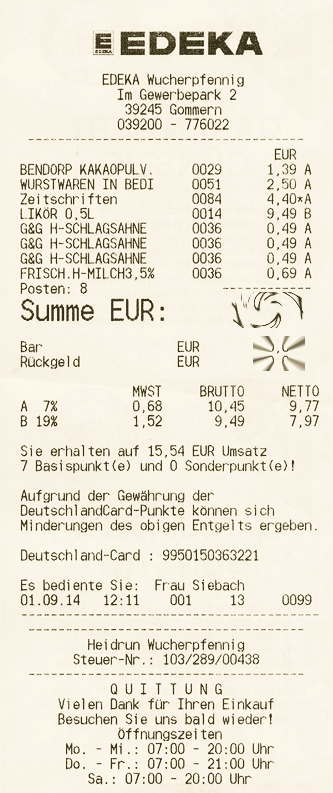
\includegraphics[height=\textwidth]{6.2-LT-Abb_Kassenzettel_1}}
		
		Auf dem Kassenzettel oben wurde der zu zahlende Betrag verwischt. Berechne die Summe des Einkaufs.
		
		\loesung{\EUR{19,94}}
	\end{karte1}

	\leereKarte

	\begin{karte2}{Kassenzettel 2}
		\begin{center}
			\rotatebox{90}{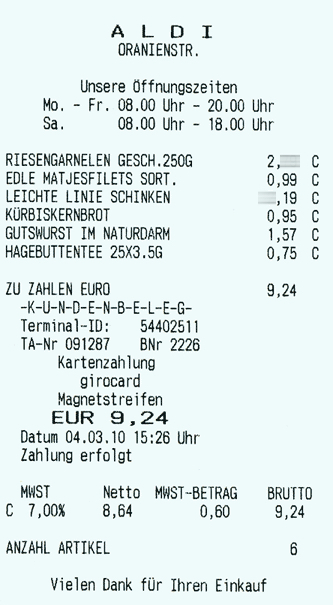
\includegraphics[height=\textheight]{6.2-LT-Abb_Kassenzettel_2}}
		\end{center}
		
		Auf dem Kassenzettel oben sind zwei Werte verwischt worden. Kannst du die fehlenden Zahlen herausfinden?
		
		\loesung{\EUR{2,79} und \EUR{2,19}}
	\end{karte2}
	
	\leereKarte

	\begin{karte3}[\symPartner]{Zahlen raten}
		Such dir für diese Karte einen Partner.
		
		\begin{multicols}{2}
			\begin{enumerate}
				\item Überlegt euch jeder \textbf{sechs} unterschiedliche Dezimalzahlen und schreibt sie auf einen Zettel.	
				\item Addiert jeder \textbf{drei} der Dezimalzahlen zusammen und notiert die Summe auf einem anderen Zettel.
				\item Tauscht beide Zettel mit eurem Partner.
				\item Versucht die drei Zahlen zu ermitteln, die zusammen die Summe ergeben.
			\end{enumerate}
			
			\columnbreak
			
			\begin{center}
				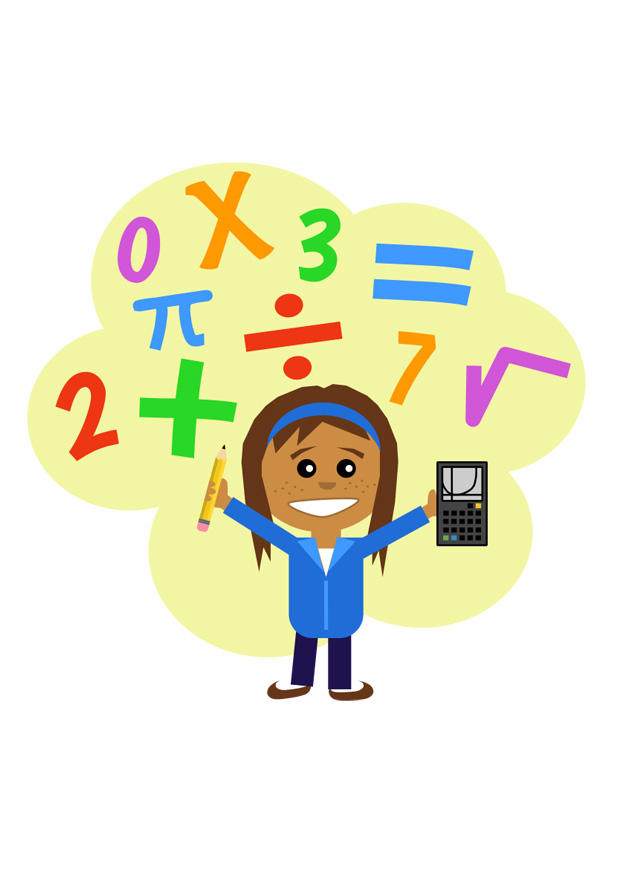
\includegraphics[width=6cm]{6.2-LT-Abb_Rechnen}
			\end{center}
		\end{multicols}
		
		\infotext{\enquote{Rechnen} von \url{http://schulbilder.org}}
	\end{karte3}
	
	\leereKarte
	
	\begin{karte2}{Druckerkabel}\hilfeMarke{addieren-und-subtrahieren}
		Der Computer von Frau Peterson soll mit dem Drucker per Kabel verbunden werden. Damit das Kabel nicht Mitten durch den Raum liegt, muss das Kabel an der Wand entlang angebracht werden.
		
		Wie viele Meter Kabel braucht Frau Peterson, wenn sie die kürzeste Strecke nutzt?
		
		\hinweis{Notiere Rechnung und Antwortsatz im Heft.}
		
		\bigskip
		\begin{center}
			\begin{tikzpicture}[x=1cm,y=1cm,scale=1.5,thick]
			\geoUrsprung;
			\geoKoordinaten{6.89/0/A,6.89/3.54/B,0/3.54/C,0/2.52/D};
			\draw[fill=gray!20] (O) |- (B) |- cycle;
			\geoAbmessung{right}(A,B){\SI{3,54}{\meter}};
			\geoAbmessung{above}(B,C){\SI{6,89}{\meter}};
			\geoAbmessung{left}(C,D){\SI{0,93}{\meter}};
			\node at (.5,2.52) []{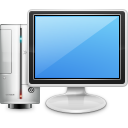
\includegraphics[width=1cm]{6.2-LT-Abb_Computer}};
			\node at (6.39,0.5) {
\includegraphics[width=1cm]{6.2-LT-Abb_Drucker}};
			\end{tikzpicture}
		\end{center}
	\end{karte2}
	
	\begin{loesungskarte}
	\begin{sachaufgabe}
		\frage Wie viele Meter Kabel braucht Frau Peterson?
		\rechnung 
		Strecke 1: $3,54 + 6,89 + 0,93 = 11,36$
		Strecke 2: $6,89 + (3,54-0,93) = 9,50$
		\antwort Für die kürzeste Strecke braucht Frau Peterson \SI{9,50}{\meter} Kabel.
	\end{sachaufgabe}
	\end{loesungskarte}

	\begin{karte3}{Die DIN-Norm}
		Ein normales BLatt hat das Format \enquote{DIN-A4}. Es hat die Breite \SI{21}{\centi\meter} und die Höhe \SI{27,9}{\centi\meter}. Legt man zwei DIN-A4 Blätter nebeneinander erhält man ein Blatt im Format \enquote{DIN-A3}. Halbiert man ein A4 Blatt, dann erhält man zwei Blätter im Format \enquote{DIN-A5}.
		
		\begin{enumeratea}
			\item Bei der DIN-Norm haben alle Formate (A3, A4, A5, ...) dasselbe \emph{Seitenverhältnis}. Das bedeutet, wenn man die Höhe durch die Breite teilt, kommt immer derselbe Wert heraus. Welcher ist das?
			\item Welche Breite und Höhe hat ein DIN-A0 Blatt? Welche ein DIN-A8 Blatt?
			\item Wie groß ist die Fläche eines DIN-A4 Blatts. 
			\item Überlege ohne zu rechnen: Wie große ist die Fläche eines DIN-A1 Blattes im Vergleich zu der des DIN-A4 Blatts?
		\end{enumeratea}
	\end{karte3}
	
	\begin{loesungskarte}
	\end{loesungskarte}
	
	\begin{karte3}[\symPartner]{Erstelle eine Lernstation}
		\hinweis{Bearbeite diese Karte erst, wenn du die \textcolor{green!55!black}{grünen} Karten fertig hast.}\bigskip
			
		\begin{wrapfigure}{r}{0pt}
			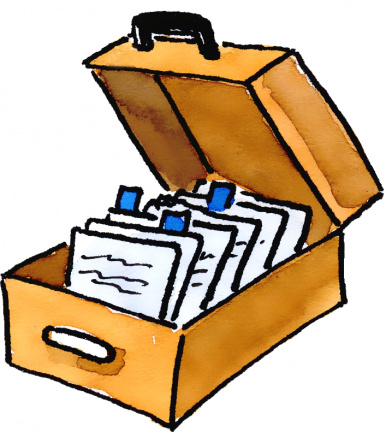
\includegraphics[width=5cm]{6.2-LT-Abb_Kartei}
		\end{wrapfigure}
		Überleg dir selber \emph{eine Lernstation} zum Thema \emph{\Titel}.
		
		Such dir zum Beispiel aus dem Buch eine Aufgabe, überlege dir mit einer Mitschülerin eine Karte oder erfinde selber eine tolle Aufgabe.
		
		Erstelle dann deine Karte auf einem Din-A5 Blatt.
		
		Deine Karte braucht auch
		\begin{smallitemize}
			\item einen Titel,
			\item eine Farbe,
			\item ein Symbol.
		\end{smallitemize}
		
		Vergiss auch nicht, auf der Rückseite \emph{die Lösung} darzustellen.
		
		\bigskip
		(\textit{Lies auf der Rückseite weiter})

		\infotext{Bild \enquote{Datenbank} von Ute Ohlms (bidab.nibis.de)}
	\end{karte3}
	
	
	\begin{karte3}{Spickzettel}
		\hinweis{Bearbeite diese Karte erst, wenn du die \textcolor{green!55!black}{grünen} Karten fertig hast.}\bigskip
			
		\begin{wrapfig}
		\begin{wrapfigure}[8]{r}{0pt}
			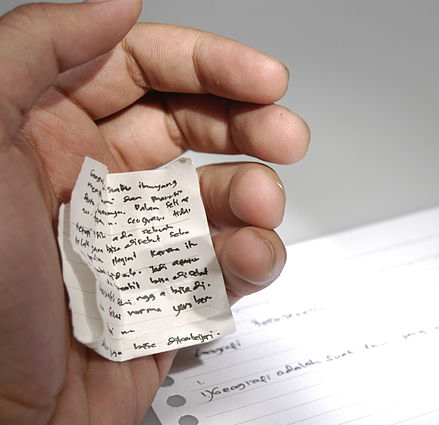
\includegraphics[width=6cm]{6.2-LT-Abb_Spicker}
		\end{wrapfigure}
		Erstelle dir einen \emph{Spickzettel} für die nächste Arbeit. Nimm dafür ein normales A4 Blatt und \emph{falte es dreimal in der Mitte}. Du hast nun ein Blatt im Format A7.
		
		
		Versuche so viele wichtige Informationen wie möglich auf ein A7 Blatt zu schreiben.
		\end{wrapfig}
		
		\infotext{Bild von Hariadhi unter CC-BY-SA-3.0}
	\end{karte3}
	
	\leereKarte
	
	\begin{karte3}[\symPartner]{Checker}
		\hinweis{Bearbeite diese Karte erst, wenn du die \textcolor{green!55!black}{grünen} Karten fertig hast.}\bigskip
		
		Erstellt euch einen \emph{Checker} (Selbstlernbogen) für die nächste Arbeit. Geht dazu so vor:
		
		\begin{enumerate}
			\item Überlegt euch, welche Themen für die Arbeit wichtig sind. Das Inhaltsverzeichnis im Buch kann dabei helfen.
			\item Sucht aus dem Buch und Arbeitsheft Aufgaben zu den Themen, die ihr zum Lernen nutzen könnt.
			\item Notiert alles in einer Tabelle.
		\end{enumerate}
		
		\begin{center}
		\begin{tabular}{c|c|c}
			\textbf{Thema} & \text{Kann ich} & \textbf{Aufgaben} \\ \hline
			Brüche in Dezimalzahlen umformen & \Large\usym{1F604}\xspace\usym{1F642}\xspace\usym{1F610}\xspace\usym{1F641} & ... \\ \hline
			& & 
		\end{tabular}
		\end{center}
	\end{karte3}
	
	\leereKarte
		
	\begin{loesungskarte}[Wenn du fertig bist]
		Wenn du mit deiner eigenen Karte fertig und zufrieden bist, dann such dir am besten einen Mitschüler, der die Karte für dich ausprobiert. Vielleicht findet er ja noch Fehler oder hat Verbesserungsvorschläge.
		
		\bigskip
		Wenn du denkst, dass deine Karte wirklich fertig ist, dann \textbf{gib sie vorne am Pult ab}.
	\end{loesungskarte}
	
\end{document}
